\pdfminorversion=7
\pdfsuppresswarningpagegroup=1
\documentclass[journal]{IEEEtran}

\usepackage[T1]{fontenc}
\usepackage[utf8]{inputenc}
\usepackage{amsmath,amssymb}
\usepackage{graphicx}
\usepackage{booktabs}
\usepackage{tabularx}
\usepackage{array}
\usepackage{url}
\usepackage[hidelinks]{hyperref}

\newcolumntype{Y}{>{\raggedright\arraybackslash}X}
\newcommand{\papertitle}{Auditing Cross-Dataset Claims in Wearable EMG Representation Learning: A Public-Data Case Study}

\begin{document}
\renewcommand{\thefigure}{S\arabic{figure}}

\title{Supplementary Material for ``\papertitle''}

\author{Anonymous~Authors}

\maketitle

\section{Supplementary Scope}
This supplement provides additional details that support the main manuscript without changing its claim boundary. The central claim remains audit-gated: representation-level signals are reported only when their semantic, diagnostic, downstream, and artifact gates are satisfied. The supplementary tables expand the related-work positioning, source-data ledger, domain-identifiability diagnostics, ontology gate, downstream baseline checks, and descriptive proxy analyses.

\section{Related-Work Claim Map}

\begin{table*}[!t]
\caption{Positioning Relative to Common Cross-Domain EMG Study Families}
\label{tab:s_relatedclaimmap}
\centering
\footnotesize
\begin{tabularx}{\textwidth}{@{}p{2.8cm}p{3.0cm}p{4.2cm}Y@{}}
\toprule
Study family & Typical claim & What the claim does not guarantee & Role of this paper \\
\midrule
Self-supervised EMG pretraining & Reusable features or improved sample efficiency & Task-valid cross-dataset supervised transfer or superiority over strong raw-feature baselines & Tests downstream claims as explicit gates rather than assuming transfer from representation learning alone \\
Domain-adversarial EMG & Lower dataset or subject identifiability & Calibrated invariance, optimal-relabel non-recoverability, or preservation of task information & Treats below-reference dataset-ID accuracy as an audit failure unless supported by balanced, relabeled, and probe diagnostics \\
OOD benchmark studies & Reported cross-subject or cross-session performance & Ontology validity across arbitrary corpora with different task definitions & Separates four-domain geometry, six-packaged-label domain-ID, and task-valid supervised endpoints \\
Large-corpus or foundation-model EMG & Aspirational reuse across devices and tasks & Clinically meaningful control transfer, fairness, or reduced recalibration burden & Requires downstream and ontology gates before deployment-facing language is allowed \\
Sensor/statistical alignment methods & Reduced feature-distribution mismatch & Shared semantic control intent or user-facing performance benefit & Treats geometry and ontology as separate prerequisites for transfer claims \\
\bottomrule
\end{tabularx}
\end{table*}

\section{Reproducibility Ledger}

\begin{table*}[!t]
\caption{Source-Data Ledger for Main Quantitative Claims}
\label{tab:s_reproledger}
\centering
\scriptsize
\begin{tabularx}{\textwidth}{@{}p{3.0cm}p{2.9cm}p{3.0cm}Y@{}}
\toprule
Claim or endpoint & Source-data folder & Unit or split & Decision boundary \\
\midrule
Training mixture counts & Canonical release tables & Packaged records & Counts are package records, not full raw-dataset sizes \\
Label-agnostic CKA shift & Canonical release tables; alignment sensitivity & Six unordered four-domain pair means plus direction-labeled source rows & Bounded pass only for small unwhitened geometry shift \\
Whitened CKA result & Canonical release tables; alignment sensitivity & Six unordered four-domain pair means plus direction-labeled source rows & Fail for whitening-invariant alignment \\
Canonical adversarial dataset-ID endpoint & Canonical release tables & Logged mini-batch readout & Failed calibration diagnostic, not invariance evidence \\
Six-packaged-domain fixed probe & Six-packaged-domain fixed-probe folder & 5 encoders $\times$ 10 probe seeds & Reject calibrated invariance for probed embeddings \\
Ontology gate & Ontology controls & Predeclared control-intent mapping & Hyser--GRABMyo transfer not evaluable \\
Downstream baseline gates & Canonical baselines; post-freeze confirmation audit & Same-subject and held-out-subject units & Classical signals can help, but pretrained feature superiority fails \\
Audit integrity & Audit checks & Frozen package checks & Supports reproducibility, not deployment readiness \\
\bottomrule
\end{tabularx}
\end{table*}

\section{Alignment Sensitivity Checks}

The released source tables retain direction-labeled source-target rows because the original sampling and reference-cluster bookkeeping were directional. Linear CKA itself is symmetric for a fixed pair of embedding matrices, so the claim-bearing summary uses reciprocal-averaged unordered pairs and leave-one-domain checks.

\begin{table*}[!t]
\caption{Unordered Four-Domain CKA Sensitivity}
\label{tab:s_unorderedcka}
\centering
\footnotesize
\begin{tabularx}{\textwidth}{@{}p{4.1cm}rrrY@{}}
\toprule
Unordered pair & Mean delta & Minimum direction & Maximum direction & Interpretation \\
\midrule
HARMONIC--NinaPro/MeganePro & +0.00416 & +0.00237 & +0.00595 & Positive in both direction-labeled source rows \\
HARMONIC--GRABMyo & +0.00491 & -0.00186 & +0.01168 & Positive pair mean, but one direction-labeled row was negative \\
HARMONIC--Hyser & +0.00244 & +0.00184 & +0.00303 & Positive in both direction-labeled source rows \\
NinaPro/MeganePro--GRABMyo & +0.00663 & +0.00231 & +0.01095 & Positive in both direction-labeled source rows \\
NinaPro/MeganePro--Hyser & +0.00220 & +0.00200 & +0.00241 & Positive in both direction-labeled source rows \\
GRABMyo--Hyser & +0.00305 & +0.00271 & +0.00339 & Positive in both direction-labeled source rows \\
\bottomrule
\end{tabularx}
\end{table*}

\begin{table*}[!t]
\caption{Leave-One-Domain CKA Sensitivity}
\label{tab:s_leaveonecka}
\centering
\footnotesize
\begin{tabularx}{\textwidth}{@{}p{3.5cm}rrrY@{}}
\toprule
Left-out domain & Mean remaining delta & Minimum direction & Maximum direction & Direction-row sign count \\
\midrule
HARMONIC & +0.00396 & +0.00200 & +0.01095 & 6 positive, 0 negative \\
NinaPro/MeganePro & +0.00347 & -0.00186 & +0.01168 & 5 positive, 1 negative \\
GRABMyo & +0.00293 & +0.00184 & +0.00595 & 6 positive, 0 negative \\
Hyser & +0.00523 & -0.00186 & +0.01168 & 5 positive, 1 negative \\
\bottomrule
\end{tabularx}
\end{table*}

These sensitivity tables support only a small unwhitened geometry shift. They do not establish whitening-invariant alignment, calibrated domain invariance, supervised semantic transfer, or downstream control benefit.

\section{Six-Domain Fixed-Probe Diagnostics}

\begin{table*}[!t]
\caption{Six-Packaged-Domain Fixed-Embedding Probe Summary}
\label{tab:s_sixdomainprobe}
\centering
\footnotesize
\begin{tabularx}{\textwidth}{@{}lrrrrrrY@{}}
\toprule
Condition & Encoders & Probe seeds/encoder & Classes & Accuracy & Balanced accuracy & Macro-F1 & Interpretation \\
\midrule
True package labels & 5 & 10 & 6 & 0.92748 & 0.92262 & 0.92086 & Package/source identity remained highly recoverable from frozen embeddings \\
Shuffled training-label control & 5 & 10 & 6 & 0.18944 & 0.18829 & 0.18446 & Control remained near the six-class reference and majority baseline \\
\bottomrule
\end{tabularx}
\end{table*}

These are independent fixed-probe diagnostics; they do not reconstruct the original adversarial-head confusion matrix, true or predicted marginals, fixed-set entropy, balanced accuracy, mutual information, optimal-relabel accuracy, or readout-training trace.

\begin{table*}[!t]
\caption{Per-Domain Recall in the Six-Packaged-Domain Fixed Probe}
\label{tab:s_sixdomainrecall}
\centering
\footnotesize
\begin{tabularx}{\textwidth}{@{}lrrrrY@{}}
\toprule
Domain & True support mean & Predicted support mean & Recall mean & Recall range & Interpretation \\
\midrule
HARMONIC & 1291.6 & 1293.22 & 1.00000 & 1.00000--1.00000 & Package stream was perfectly recoverable; see boundary below \\
NinaPro DB10/MeganePro & 1249.9 & 1249.98 & 0.99962 & 0.99759--1.00000 & Primary feature-bank domain was nearly perfectly recoverable \\
PhysioNet GRABMyo & 1270.9 & 1271.40 & 0.99972 & 0.99841--1.00000 & Primary feature-bank domain was nearly perfectly recoverable \\
PhysioNet Hyser & 1247.3 & 1257.76 & 0.99992 & 0.99920--1.00000 & Primary feature-bank domain was nearly perfectly recoverable \\
emg2pose & 1333.3 & 1267.70 & 0.77639 & 0.69685--0.86464 & Limited indexed subset; lower recoverability than primary domains \\
emg2qwerty & 966.8 & 1019.74 & 0.76007 & 0.51157--0.88505 & Limited indexed subset; lower recoverability than primary domains \\
\bottomrule
\end{tabularx}
\end{table*}

For HARMONIC, the rebuilt six-packaged-domain probe used a reconstructed public text/probability stream rather than raw HARMONIC EMG. Perfect recall therefore shows package-stream recoverability, not raw-EMG physiological separability.

\section{Ontology Gate}

\begin{table*}[!t]
\caption{Ontology-Gate Decisions}
\label{tab:s_ontology}
\centering
\footnotesize
\begin{tabularx}{\textwidth}{@{}p{3.0cm}p{2.3cm}p{2.3cm}ccY@{}}
\toprule
Endpoint & Source & Target & Accepted classes & Allowed? & Permitted wording \\
\midrule
GRABMyo same-dataset session shift & GRABMyo & GRABMyo & 17 & Yes & Same-dataset task-valid screen \\
Hyser same-dataset session shift & Hyser & Hyser & 34 & Yes & Same-dataset task-valid screen \\
Hyser to GRABMyo supervised transfer & Hyser & GRABMyo & 0 & No & Not evaluable; no documented one-to-one control-intent mapping exposed by frozen package \\
GRABMyo to Hyser supervised transfer & GRABMyo & Hyser & 0 & No & Not evaluable; no documented one-to-one control-intent mapping exposed by frozen package \\
\bottomrule
\end{tabularx}
\end{table*}

\section{Downstream Baseline Sensitivity}

\begin{table*}[!t]
\caption{Downstream Baseline Checks Used as Claim-Inclusion Gates}
\label{tab:s_baselines}
\centering
\footnotesize
\begin{tabularx}{\textwidth}{@{}p{3.0cm}p{4.0cm}p{3.0cm}Y@{}}
\toprule
Screen & Comparison & Effect & Gate interpretation \\
\midrule
Same-subject frequency comparator & Raw + pretrained vs. raw + frequency & $-0.03516$ normalized log-AULC & Conventional frequency comparator did not rescue a pretrained-feature advantage \\
Same-subject frequency comparator & Frequency-only vs. raw statistics & $-0.00425$ normalized log-AULC & Frequency features were close to raw statistics but did not beat them overall \\
Held-out-subject classical signal comparator & Classical + pretrained vs. classical & +0.00605 normalized log-AULC; sign-flip $p=0.16242$ & Below effect threshold, dataset-heterogeneous, and failed positive gate \\
Held-out-subject classical signal positive control & Raw + classical signal features vs. raw statistics & +0.0837 normalized log-AULC in main manuscript & Offline GRABMyo/Hyser ridge-readout screen detected useful classical signal-feature information under this constrained benchmark; not an online-control, EMGBench, or state-of-the-art baseline-suite result \\
\bottomrule
\end{tabularx}
\end{table*}

\begin{figure*}[!t]
\centering
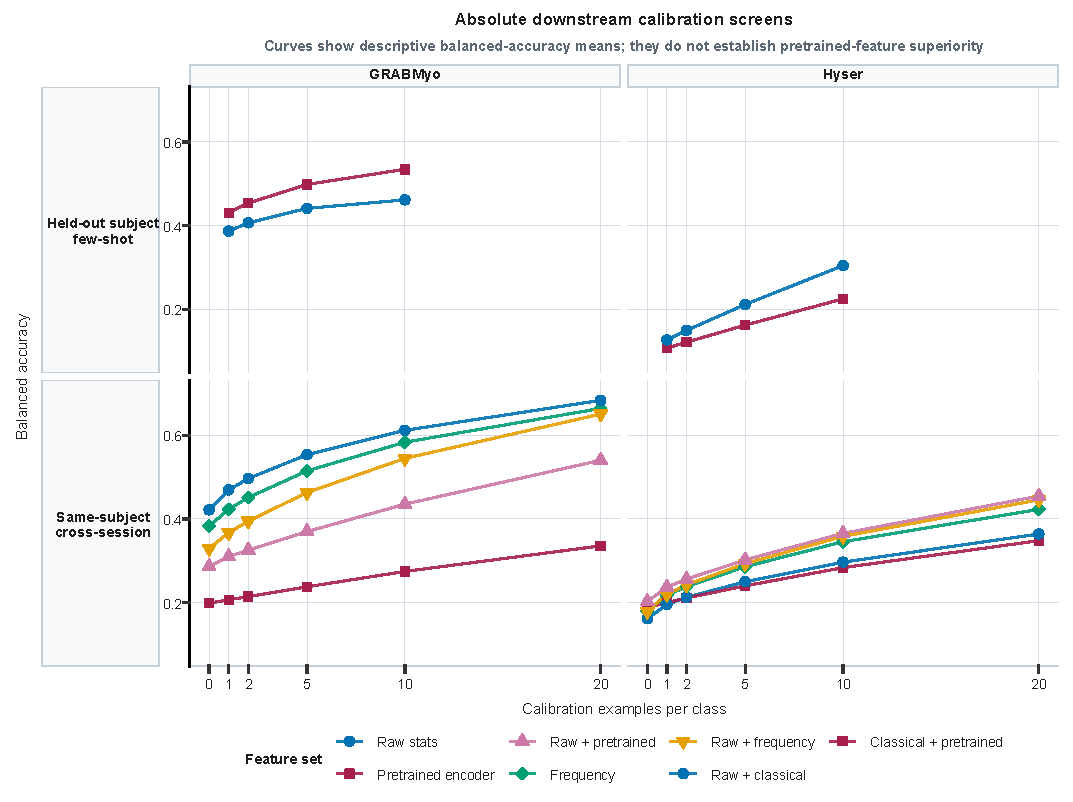
\includegraphics[width=\textwidth]{figures_compiled/figS05_downstream_absolute_accuracy_curves.pdf}
\caption{Absolute downstream balanced-accuracy curves for the claim-inclusion screens. Panels show absolute accuracy across calibration counts rather than only normalized log-AULC deltas. The curves confirm that pretrained features did not establish superiority over raw statistics or classical signal features under these offline ridge-readout screens.}
\label{fig:s_absolute_downstream}
\end{figure*}

\section{Descriptive Proxy Analyses}

\begin{figure*}[!t]
\centering
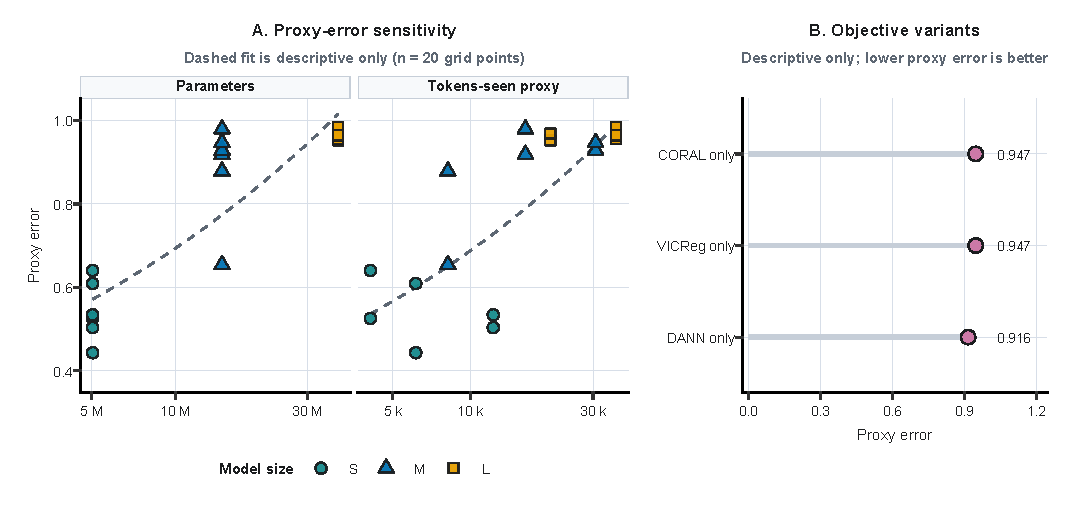
\includegraphics[width=\textwidth]{figures_compiled/figS04_scaling_ablation_descriptive.pdf}
\caption{Descriptive frozen-grid size-sensitivity and objective-ablation summaries. Lower frozen-grid proxy error is better. The log-log fits were computed against the tokens-seen proxy and parameter count across the small, medium, and large settings evaluated in the core grid, and the objective-ablation panel reports the available frozen-ledger component runs. These summaries are descriptive and should not be read as a universal EMG scaling law, causal objective proof, or supervised cross-dataset transfer evidence.}
\label{fig:s_scaling}
\end{figure*}


\section{Additional Provenance and Diagnostic Material Moved from Main Text}
The following ledgers and diagnostic figures were moved from the main manuscript to reduce main-text density while preserving reviewer access to the full audit trail.

\begin{figure*}[t]
\centering
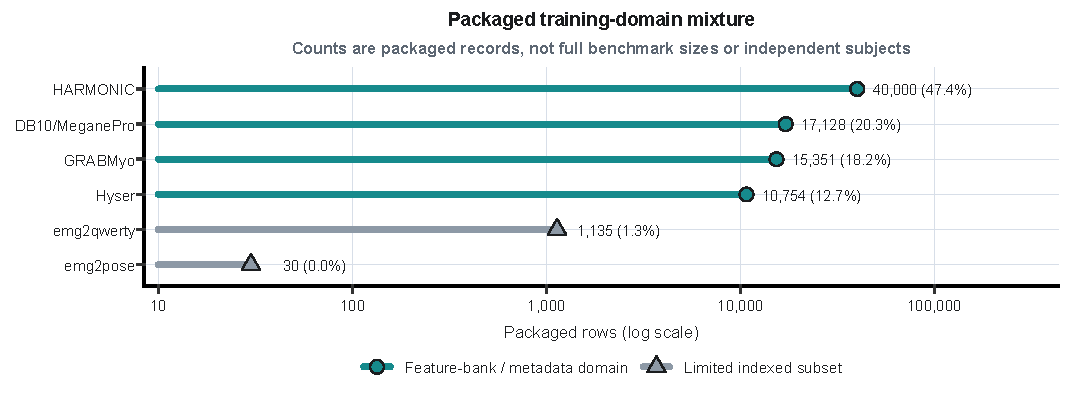
\includegraphics[width=\textwidth]{figures_compiled/figS01_training_domain_mixture.pdf}
\caption{Training-domain mixture used by the canonical audited package. The pretraining corpus was dominated by HARMONIC, NinaPro DB10 plus MeganePro, PhysioNet GRABMyo, and PhysioNet Hyser, with emg2qwerty and emg2pose contributing much smaller limited indexed subsets. These limited indexed subsets should not be interpreted as full emg2qwerty or emg2pose benchmark evaluation.}
\label{fig:trainingmixture}
\end{figure*}

\begin{table*}[t]
\caption{Prepared-Package Reproducibility Ledger}
\label{tab:packagerepro}
\centering
\footnotesize
\begin{tabularx}{\textwidth}{@{}p{2.35cm}p{2.25cm}p{1.65cm}p{2.15cm}p{2.65cm}Y@{}}
\toprule
Packaged domain & Source role & Records used & Canonical input & Main evaluation role & Claim boundary \\
\midrule
HARMONIC & Multimodal collaboration / stress-test data & 40{,}000 & 16 channels $\times$ 64 samples & Four-domain feature-bank alignment; six-label readout and six-packaged-domain fixed-probe diagnostics & Packaged records; in the rebuilt six-packaged-domain probe, HARMONIC was reconstructed from the public text/probability stream rather than raw EMG \\
NinaPro DB10 + MeganePro & Prosthetic grasp-intent feature bank & 17{,}128 & 16 channels $\times$ 64 samples & Four-domain feature-bank alignment; six-label readout and six-packaged-domain fixed-probe diagnostics & Combined feature-bank domain; not a standalone DB10 benchmark result \\
PhysioNet GRABMyo & Multi-day gesture / biometric EMG & 15{,}351 & 16 channels $\times$ 64 samples & Four-domain alignment; same-dataset calibration screen; ontology gate; fixed-probe diagnostics & Transfer to Hyser blocked unless control-intent equivalence is documented \\
PhysioNet Hyser & HD-sEMG manipulation / neural-interface resource & 10{,}754 & 16 channels $\times$ 64 samples & Four-domain alignment; same-dataset calibration screen; ontology gate; fixed-probe diagnostics & HD-sEMG topology and richer temporal structure are compressed by canonicalization \\
emg2qwerty & Limited indexed pretraining subset & 1{,}135 & 16 channels $\times$ 64 samples & Six-label mixture and post-freeze fixed-probe diagnostics & Limited 86-file, 10-subject indexed subset in the rebuilt probe; not full emg2qwerty benchmark utilization \\
emg2pose & Limited indexed pretraining subset & 30 & 16 channels $\times$ 64 samples & Six-label mixture and post-freeze fixed-probe diagnostics & Mini subset with trial/file-level splitting; too small for independent alignment or downstream claims \\
\bottomrule
\end{tabularx}
\end{table*}

\begin{table*}[t]
\caption{Analysis Provenance and Claim Boundary}
\label{tab:analysisprovenance}
\centering
\footnotesize
\begin{tabularx}{\textwidth}{@{}p{3.1cm}p{4.1cm}p{4.4cm}Y@{}}
\toprule
Analysis block & Artifact status & Used for & Not used for \\
\midrule
Canonical frozen package & Frozen before final interpretation; primary geometry, logged domain-ID, ontology, scaling, ablation, and integrity endpoints were read from saved artifacts & Primary audit case study and claim-gate ledger & Post-freeze model selection, architecture tuning, or converting failed gates into positive claims \\
Post-freeze domain-ID confirmation & Five independently seeded medium encoders, each evaluated with ten grouped probe seeds on all six packaged labels & Testing whether package/source identity remained recoverable from trained embeddings after the canonical readout failed near-reference calibration & Reconstructing the missing six-label adversarial head, claiming full emg2qwerty/emg2pose benchmark use, or proving physiological domain equivalence \\
Post-freeze downstream screens & Same-dataset session and held-out-subject ridge-readout screens with raw, pretrained, and classical signal-feature comparators & Testing whether a task-valid pretrained-feature-superiority or reduced-calibration claim passed conservative gates & Claiming online control, clinical deployment, EMGBench leaderboard performance, or universal baseline superiority \\
Reproducibility package & Public GitHub release, manuscript source data, source-table checksums, and separate complete result archive & Independent tracing of figure/table values and confirmation artifacts & Redistribution of raw third-party EMG datasets or replacement of provider access terms \\
\bottomrule
\end{tabularx}
\end{table*}

\begin{table*}[t]
\caption{Split and Leakage Controls by Endpoint}
\label{tab:splitleakage}
\centering
\footnotesize
\begin{tabularx}{\textwidth}{@{}p{3.0cm}p{3.8cm}p{4.2cm}Y@{}}
\toprule
Endpoint & Split unit & Leakage control & Boundary \\
\midrule
Frozen representation package & Subject-wise validation splits where subject identifiers were available; mixed-domain self-supervised batches & Subject-overlap and forbidden-token audit tables report zero overlap or sentinel hits for the frozen subject-held-out partitions & Self-supervised pretraining is not itself a clinical test split and does not establish task-valid control transfer \\
Same-subject cross-session screen & Earliest session as source and later sessions as target within each subject & Calibration and evaluation were within a subject across sessions; this intentionally probes session shift, not subject independence & Not evidence of new-subject generalization \\
Held-out-subject few-shot screen & Held-out subject as target; source data from other subjects in the same dataset & Calibration windows and test windows for the held-out subject were trial-blocked where trial identifiers were available & Still an offline ridge-readout screen rather than online control \\
Fixed-embedding package/source-ID probes & Grouped logistic-regression probe seeds on frozen embeddings; subject-level where available and trial/file-level for emg2pose & Shuffled training-label controls and prediction-level confusion/support summaries were produced for all six packaged labels & Does not reconstruct the missing adversarial readout or create full emg2qwerty/emg2pose benchmark claims \\
Artifact-integrity audit & Saved source tables, manifests, recomputation checks, and checksum ledgers & Subject-overlap, feature-sentinel, permutation-margin, and recomputation-consistency checks are included in source data & Aggregate checks do not expose every raw trial ID because raw third-party data are not redistributed \\
\bottomrule
\end{tabularx}
\end{table*}

\begin{table*}[t]
\caption{Domain-Identifiability Audit Ledger}
\label{tab:domainiddiagnostics}
\centering
\footnotesize
\begin{tabularx}{\textwidth}{@{}p{3.0cm}p{4.25cm}p{4.25cm}Y@{}}
\toprule
Endpoint & Observed evidence & Missing diagnostic requirement & Audit interpretation \\
\midrule
Logged readout, step 5 & Accuracy 0.3398; entropy 1.4912; active domains: emg2qwerty, HARMONIC, GRABMyo & Held-out all-six confusion, supports, marginals, balanced accuracy, optimal relabeling, and mutual information & Aggregate mini-batch readout, not six-packaged-domain recoverability \\
Logged readout, step 10 & Accuracy 0.1211; entropy 1.3303; active domains: emg2pose, emg2qwerty, GRABMyo & Same as above & Intermediate below-reference logged readout \\
Logged readout, step 15 & Accuracy 0.0234; entropy 1.4749; active domains: emg2qwerty, HARMONIC, NinaPro/MeganePro & Same as above & Failed near-reference calibration check; mechanism unresolved \\
Post-freeze six-packaged-domain fixed probe & Five encoders $\times$ ten probe seeds recovered six packaged-domain identity with balanced accuracy 0.92262; shuffled-control balanced accuracy was 0.18829 & Does not reconstruct the original adversarial readout; limited emg2pose/emg2qwerty subsets are not full benchmarks & Package/source identity remained recoverable from frozen embeddings \\
Remaining canonical adversarial diagnostics & No original-head six-by-six held-out confusion matrix, true supports, predicted marginals, entropy on fixed all-domain set, six-label optimal-relabel accuracy, or adversarial readout trace was exposed by the canonical artifact & Required before explaining the 0.0234 adversarial-head mechanism & The 0.0234 endpoint cannot certify invariance \\
\bottomrule
\end{tabularx}
\end{table*}

\begin{figure*}[t]
\centering
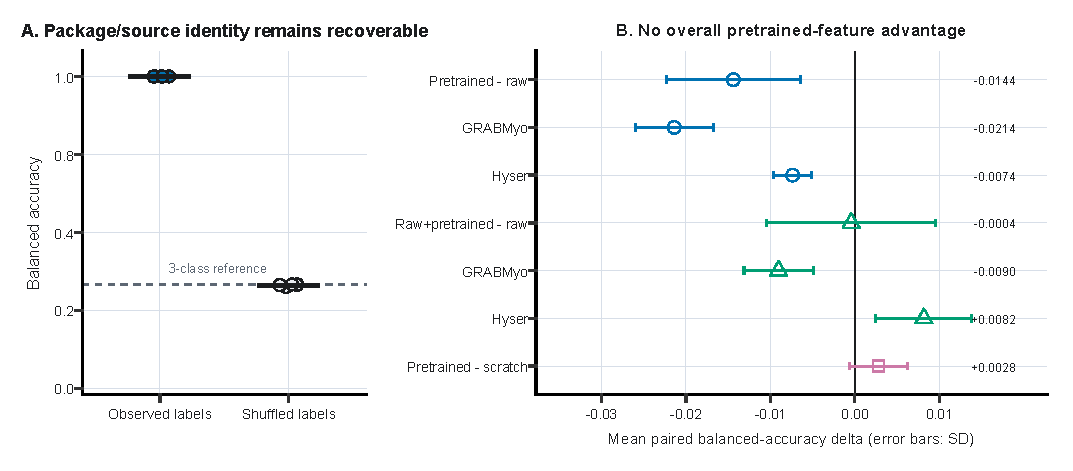
\includegraphics[width=\textwidth]{figures_compiled/fig08_confirmatory_audit.pdf}
\caption{Post-freeze confirmation diagnostics. (A) Independent subject-held-out package/source-ID probes across five seeded medium encoders and ten probe seeds per encoder recovered three-source identity from frozen embeddings with mean balanced accuracy 0.99989; shuffled-label controls were near the three-class reference at 0.33069. The main-text post-freeze probe table extends this recoverability diagnostic to all six packaged labels. (B) Source-plus-calibration downstream paired balanced-accuracy deltas did not establish a pretrained-feature advantage: pretrained-minus-raw was negative overall, and raw-plus-pretrained minus raw was approximately neutral overall with negative GRABMyo and positive Hyser components. Error bars show encoder-level standard deviation over the summarized cells.}
\label{fig:confirmatoryaudit}
\end{figure*}

\begin{figure*}[t]
\centering
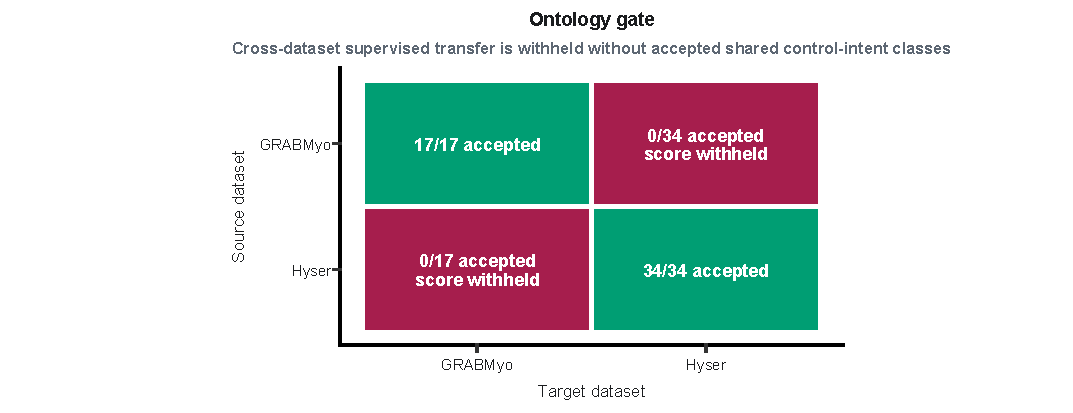
\includegraphics[width=\textwidth]{figures_compiled/figS02_ontology_gate.pdf}
\caption{Fail-closed ontology-gate summary for Hyser and GRABMyo. Because the gate found zero accepted shared control-intent classes, the package withheld a supervised transfer score rather than reporting an invalid comparison.}
\label{fig:transferfailclosed}
\end{figure*}

\begin{figure*}[t]
\centering
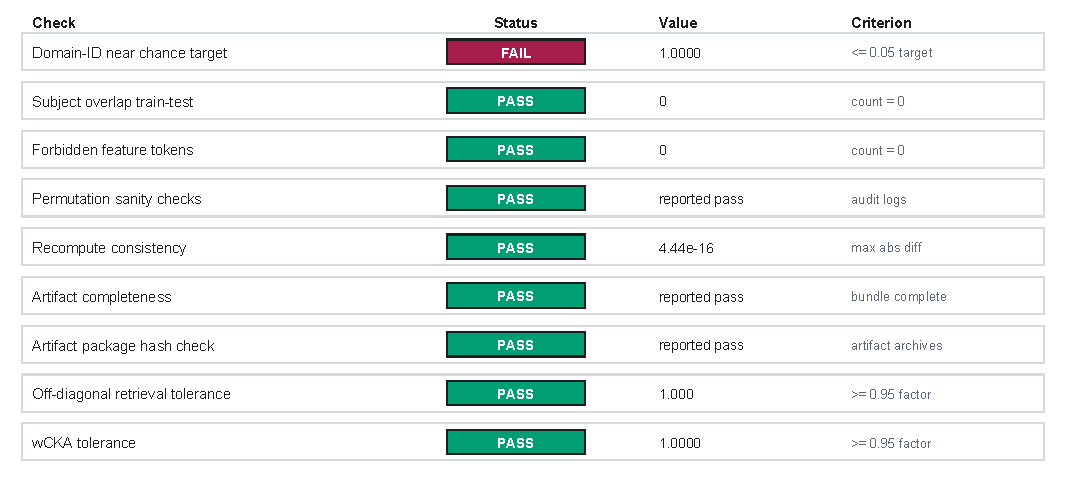
\includegraphics[width=\textwidth]{figures_compiled/figS03_artifact_integrity_checks.pdf}
\caption{Audit-integrity ledger for the frozen package. The near-reference target check failed, while subject-overlap, forbidden-token, permutation-margin, recomputation-consistency, off-diagonal retrieval, and wCKA tolerance checks passed. The wCKA tolerance check indicates non-catastrophic retention under the package threshold, not an improvement in wCKA.}
\label{fig:auditintegrity}
\end{figure*}

\section{Archive Boundary}
The review source package includes manuscript-ready CSV/JSON summaries, figures, checksums, and this supplement. It intentionally excludes raw third-party EMG data, model checkpoints, embedding caches, raw-window feature parquet files, trial-level prediction caches, local launcher logs, machine-local paths, and public repository or archive identifiers. The package supplied through the review system is self-contained and includes regenerated PDFs, source data, figures, manifest, and checksum ledger.

\end{document}
